\chapter{Installation and Manipulation of MongoDB}
%Intro\footnotemark\\
\par In this Chapter, we will install the package provided by the ubuntu community which features the most recent version.

\begin{spacing}{1.2}
%note en bas de page
\section{Installation and configuration }
\par First, we import the GPK key for the "MongoDB apt Repository" on our system using the
next command.
\\
\begin{figure}[!htb] 
\begin{center} 
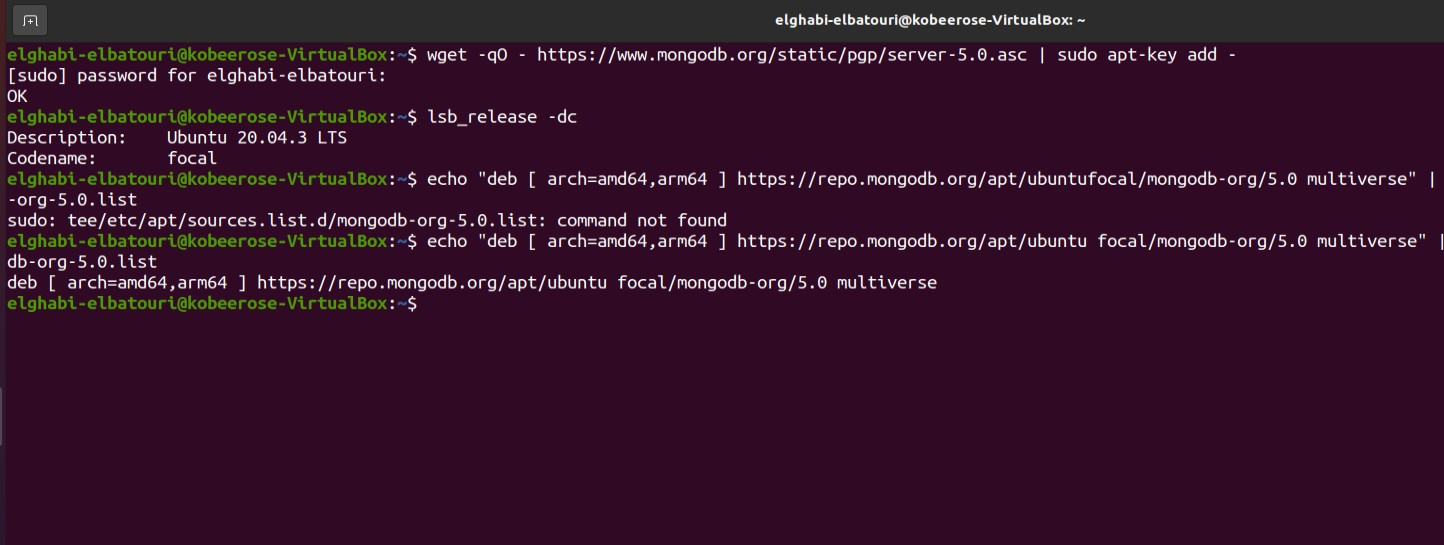
\includegraphics[width=1\linewidth]{Pictures/MongoDB/Installation and manipulation of MongoDB/Installation and configuration/Configuring the apt Repository} 
\end{center} 
\caption{Configuring the apt Repository} 
\end{figure}  \FloatBarrier
\\
\newpage
\par After adding the required “apt Repository”, we will install
MongoDB on our VM. which will also install any dependent packages required for MongoDB.
\\
\begin{figure}[!htb] 
\begin{center} 
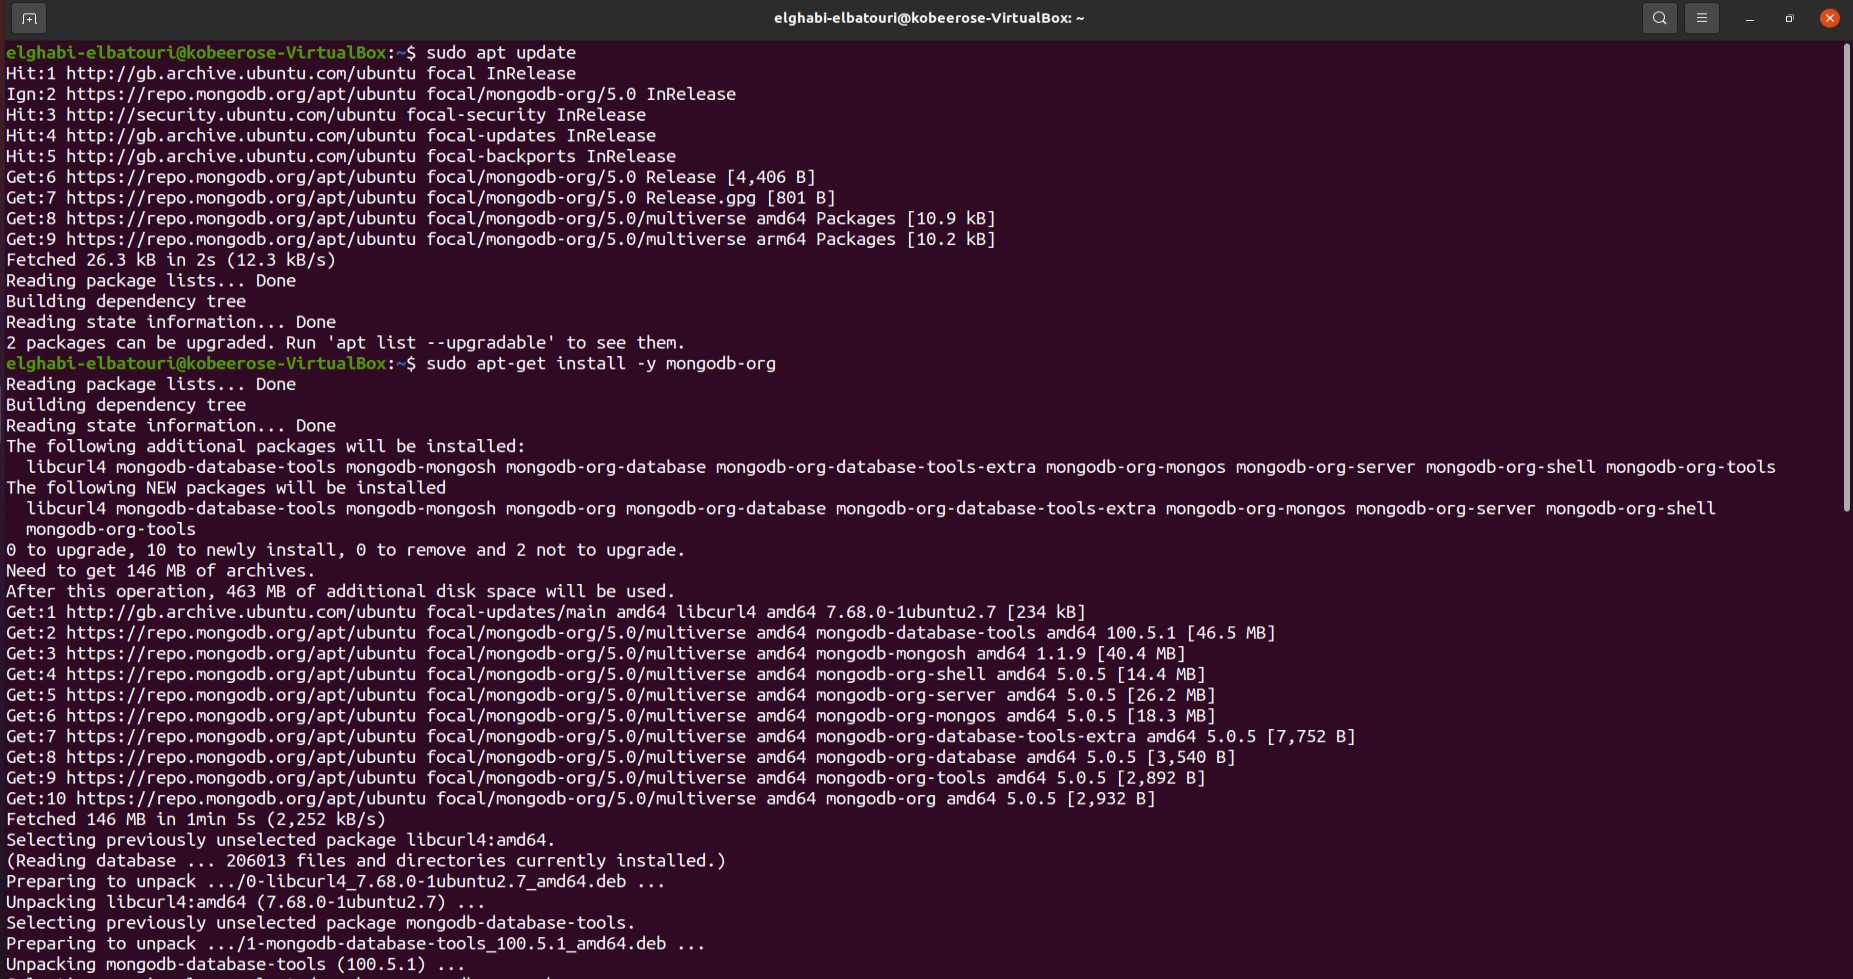
\includegraphics[width=1\linewidth]{Pictures/MongoDB/Installation and manipulation of MongoDB/Installation and configuration/Installing MongoDB} 
\end{center} 
\caption{Installing MongoDB} 
\end{figure}  \FloatBarrier
\\

\par Viewing the Version of MongoDB
\\
\begin{figure}[!htb] 
\begin{center} 
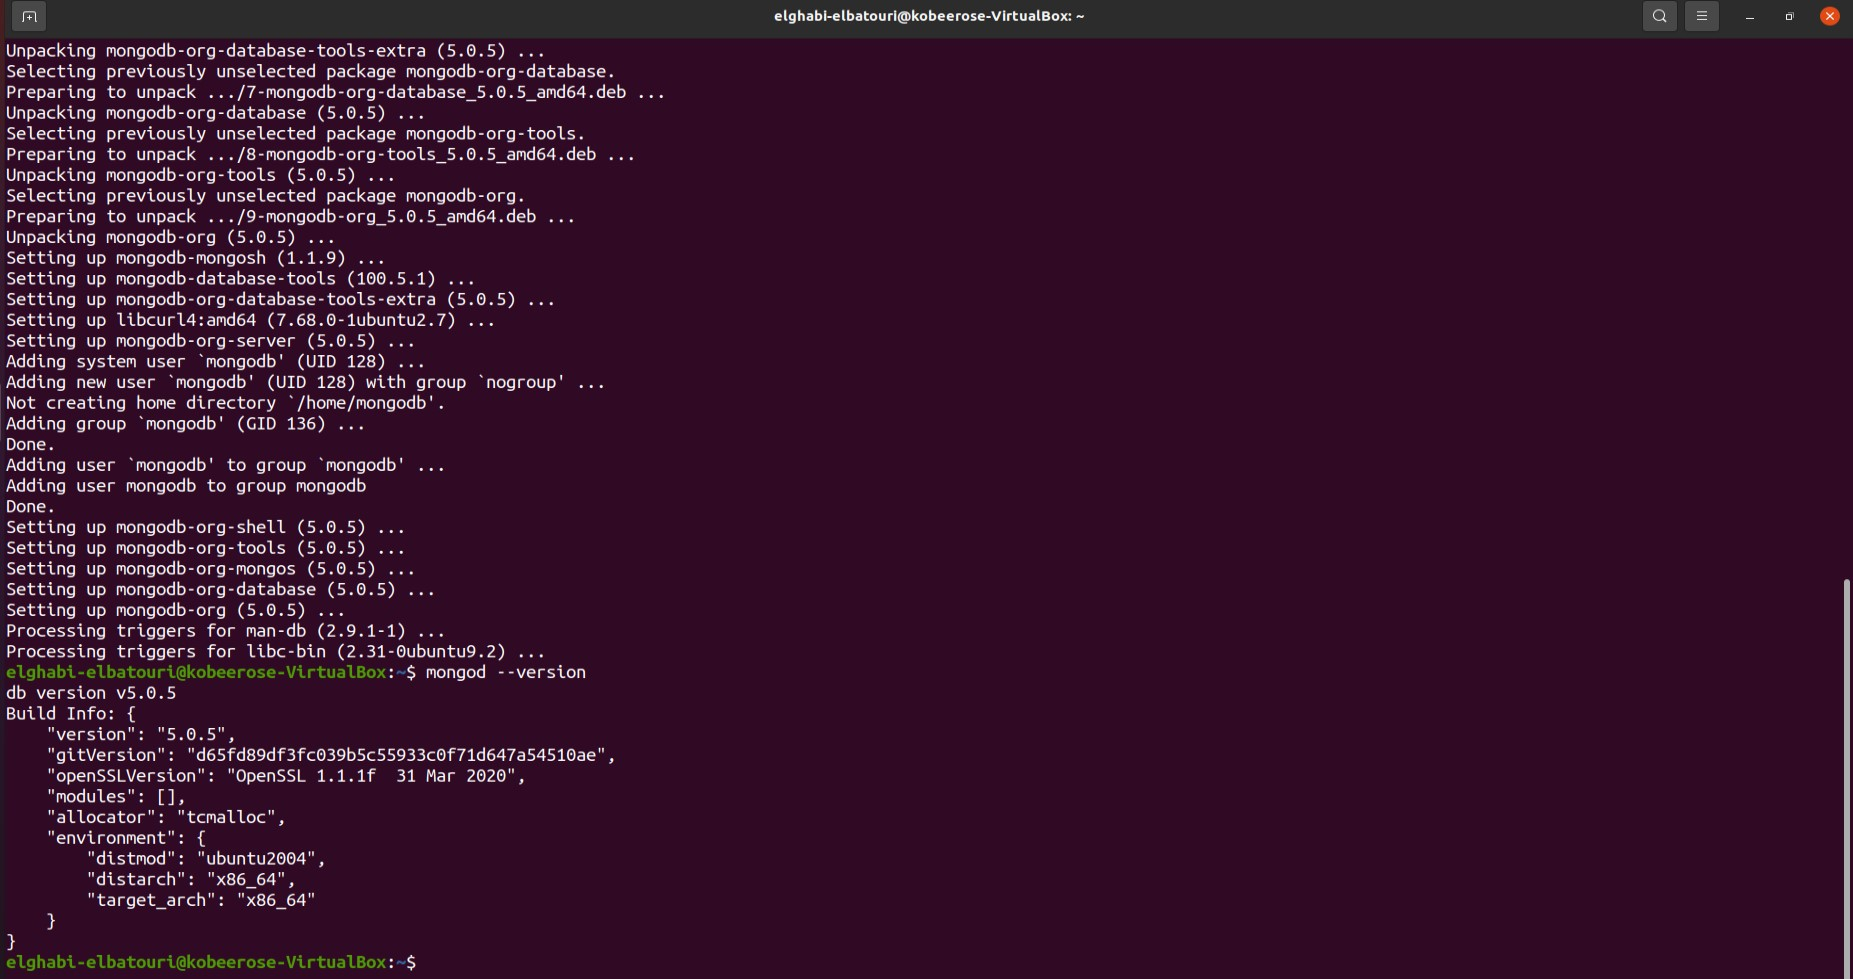
\includegraphics[width=1\linewidth]{Pictures/MongoDB/Installation and manipulation of MongoDB/Installation and configuration/Display MongoDb version} 
\end{center} 
\caption{Display MongoDb version} 
\end{figure}  \FloatBarrier
\\

\section{Mongodb service management }
\par Now, we head on to enabling and starting the services of MongoDB.
\\
\begin{figure}[!htb] 
\begin{center} 
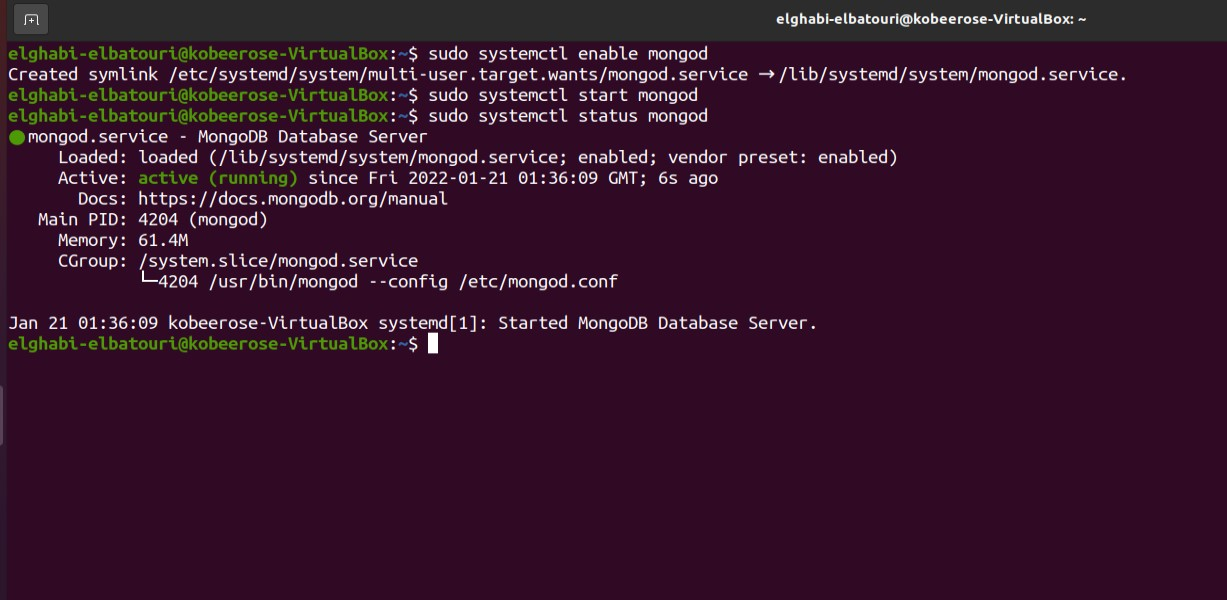
\includegraphics[width=1\linewidth]{Pictures/MongoDB/Installation and manipulation of MongoDB/Mongodb service management/activating MongoDB services} 
\end{center} 
\caption{Activating MongoDB services} 
\end{figure}  \FloatBarrier
\\

\par Let's Stop and restart the MongoDB service.a
\\
\begin{figure}[!htb] 
\begin{center} 
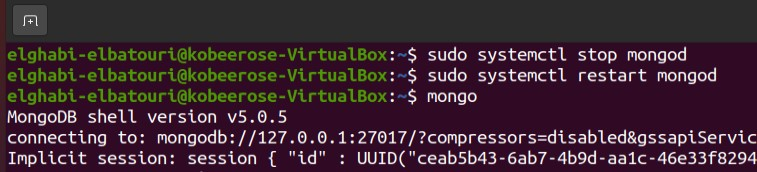
\includegraphics[width=1\linewidth]{Pictures/MongoDB/Installation and manipulation of MongoDB/Mongodb service management/restarting MongoDB service} 
\end{center} 
\caption{Restarting MongoDB service} 
\end{figure}  \FloatBarrier
\\
\newpage
\par Connecting to MongoDB using the command line and running some test commands to
check for proper operation.
\\
\begin{figure}[!htb] 
\begin{center} 
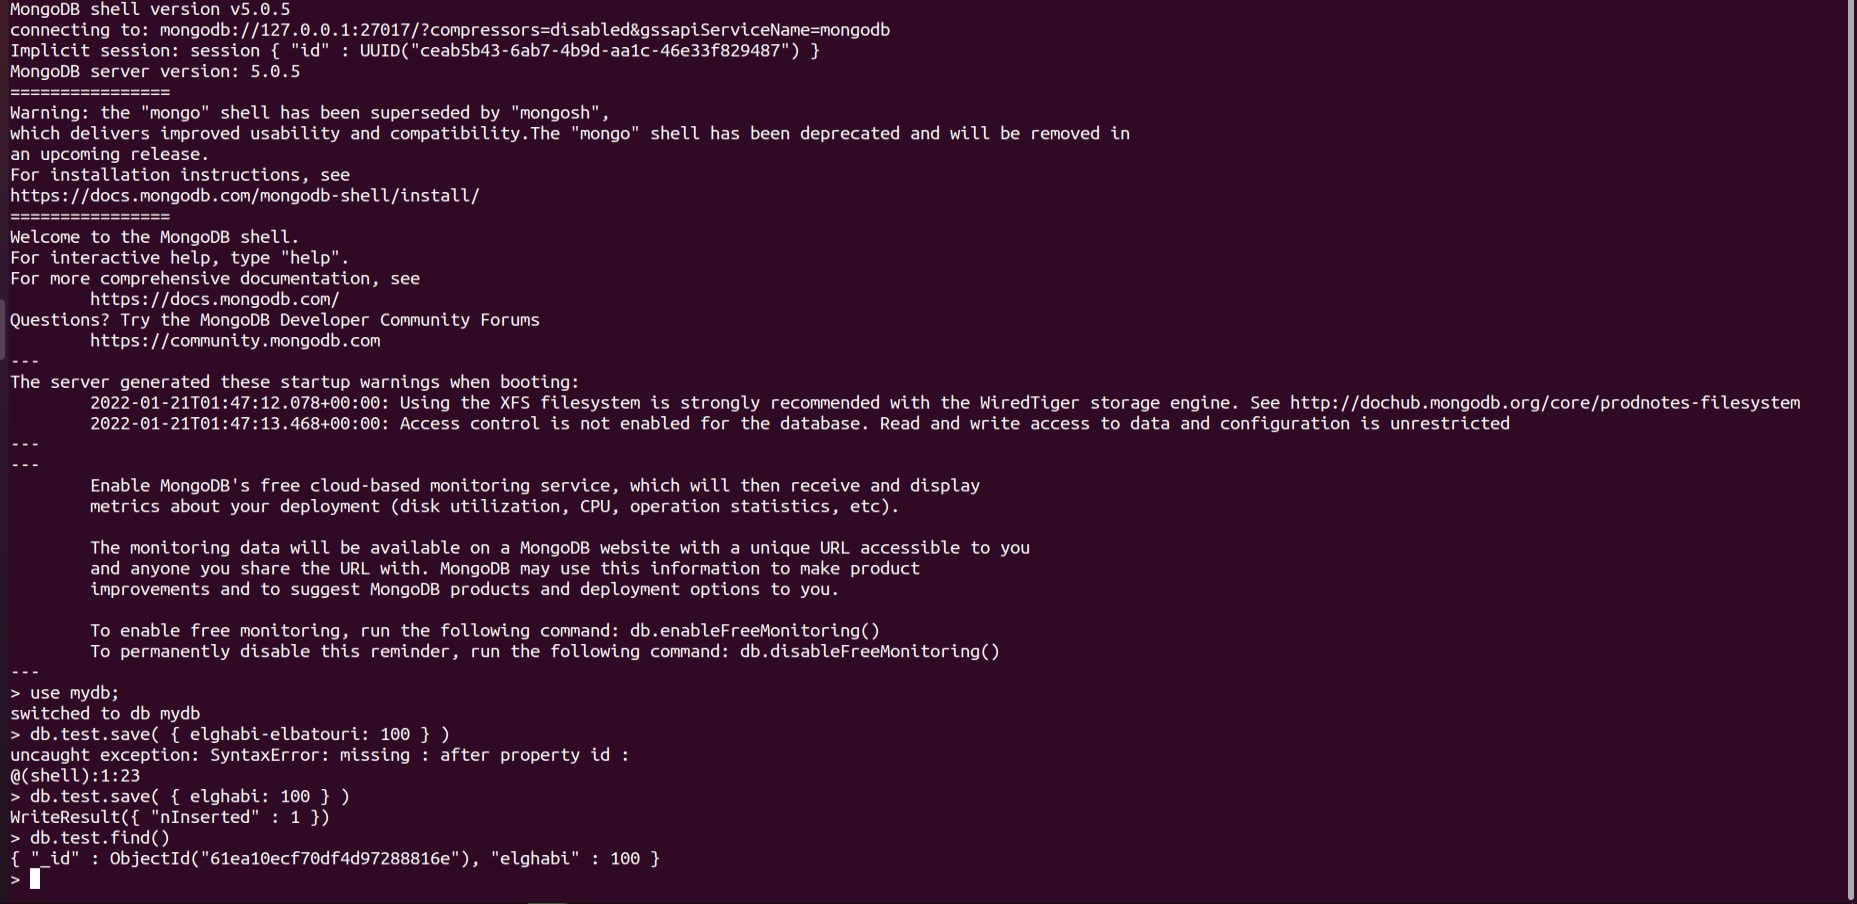
\includegraphics[width=1\linewidth]{Pictures/MongoDB/Installation and manipulation of MongoDB/Mongodb service management/configuration test} 
\end{center} 
\caption{Configuration test} 
\end{figure}  \FloatBarrier
\\

\end{spacing}